%\documentclass{article}
%\usepackage{graphicx,subfigure}
%\begin{document}

\begin{figure}[h]
  \centering
  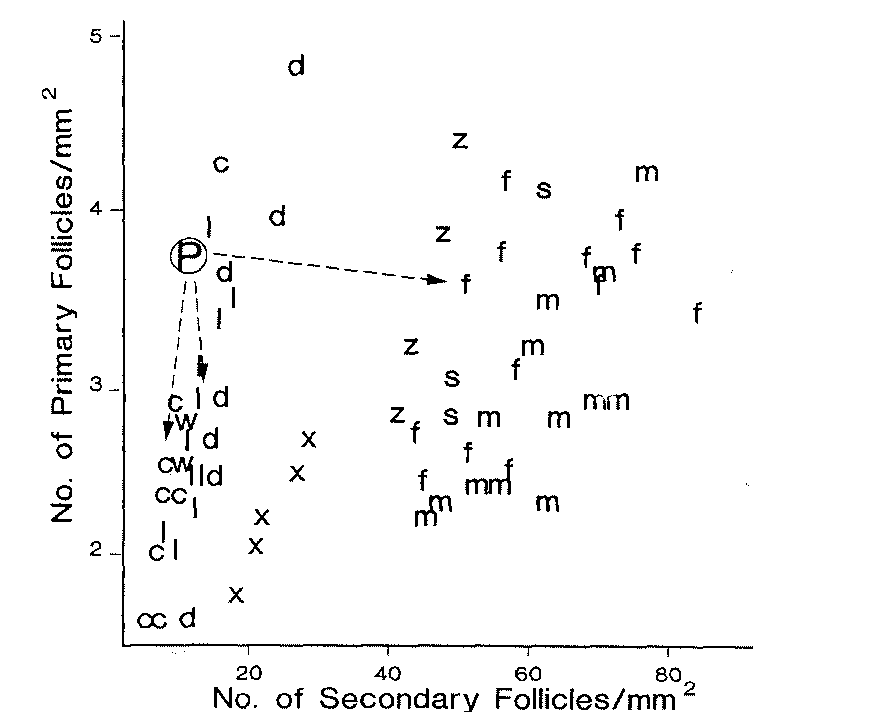
\includegraphics[width=1.3\textwidth, trim = 80 0 0 120]{images/fig6ri.png}
  \caption{ Relationship of primary fibre density (Np) to secondary fibre
      density (Ns) across a range of breeds.  Data from Carter (1968)
      and CSIRO unpublished.  Suggested lines of evolution of major
      breeds shown $-\ -\ -\ ->$. 
      Letter codes for breeds as in Figure~\ref{fig:5}.}
  \label{fig:6}
\end{figure}

%\end{document}
